\documentclass[a4paper,11pt,twoside,openright]{book}


\usepackage[utf8]{inputenc}
%\usepackage[vietnam.english]{babel}

\usepackage[T1]{fontenc}




%\usepackage[Latin1]{inputenc}       %caractËres accentuÈs et autres
%\usepackage[T1]{fontenc}            %cÈsure des mots accentuÈs
%\usepackage[frenchb]{babel}         %francisation (chapitre,annexe,rÈfÈrences...)
\usepackage{graphicx}               %insertion graphiques

\usepackage{a4wide}
%\usepackage{psfig}


%\psfigurepath{}




%\usepackage{times}


%\input{transfig}



\renewcommand{\thefootnote}{}

%% Necessaire pour creer les index
\usepackage{makeidx}
\makeindex





%%%%%%%%%%%%%%%%%%%%%%%%%%%%%%
%%%% MODIFY THIS PART FOR THE FIRST PAGE

% change the master level 
\def\MasterLevel{Master Thesis }
%\def\MasterLevel{Master 1}

\def\InternshipTitle{NOISE EVALUATION AND REDUCTION}
\def\FirstName{HOANG DUC}
\def\LastName{VIET}
\def\HostOrganization{ICTLab - USTH }
\def\CityName{Ha Noi}
\def\CountryName{Viet Nam}
\def\UniversityName{University of Science and Technology of Hanoi(USTH)}
\def\Supervisor{Ph.D Tran Giang Son}



\setlength{\textwidth}{175mm}
%
\setlength{\textheight}{245mm}

\setlength{\topmargin}{-10mm}

\setlength{\evensidemargin}{-8mm}

\setlength{\oddsidemargin}{-8mm}

% ----------------------- DEBUT DOCUMENT ---------------------------
\usepackage{amsmath}
\usepackage{listings}
\lstset{language=Matlab}
\lstset{tabsize=2}
\usepackage{caption}
\usepackage{subcaption}
\usepackage{multirow}

\begin{document}



\pagestyle{plain}



\pagenumbering{Roman}


% ----------------- DEFINITION DU TITRE ET DES AUTEURS ---------------------------

\empty
\thispagestyle{empty}

\begin{center}


\includegraphics[angle=0,width=5cm]{images/logo-1_39.png}

\vspace*{1cm} 

{\huge University of Science and Technology of Hanoi }\\

\vspace*{1cm} 

{\large Information and Communication Technology Department}\\

\vspace*{1cm} 

{\huge \MasterLevel }\\

\vspace*{1cm} 

{\large Academic year 2016 -  2017}

\vfill

\noindent\hrulefill

\vspace*{2mm} 

{\Large \InternshipTitle }

\noindent\hrulefill

\vfill 

{\large presented by } \\

\vspace*{5mm} 

{\large \bf \FirstName~  \LastName} \\

\vspace*{5mm} 

{\large registered at \UniversityName } \\

\vspace*{5mm} 

{\large supervised by  \Supervisor } \\

\vspace*{20mm} 

{\large Host organization :   \HostOrganization }

\vspace*{5mm} 

{\large  \CityName~- \CountryName} \\

\vspace*{5mm} 

\end{center}



\let\cleardoublepage\clearpage
% ----------------------- PAGE VIDE ---------------------------




\chapter*{ATTESTATION}



\vfill


\noindent\hrulefill

~\\


I hereby,  \FirstName~  \LastName, certify that my report doesn't contain plagiarism (copy/paste) from other sources.

~\\

In case of plagiarism in my report, I know the consequences and I understand that my report won't be evaluated. In this case, my M2 internship will be noted as "fail".


~\\

 Date 15/09/2017 

~\\
 
 Signature
 \FirstName~  \LastName
 

~\\
~\\
~\\
~\\
~\\

\noindent\hrulefill


\vfill


\vfill



%\selectlanguage{vietnam}
%
%
%Tôi ký tên dưới đây, <họ> <tên>, xác nhận rằng bài báo cáo của tôi không có đạo văn (lỗi sao chép) từ các nguồn khác.
%
%
%~\\
%
%
%Nếu bị phát hiện ra trong bài báo cáo, tôi biết hậu quả và tôi hiểu rằng bài báo cáo của tôi sẽ không được chấp nhận. 
%Trong trường hợp đó, học phần (thực tập năm thứ nhất, thực tập năm thứ hai, hay học phần đánh giá) sẽ bị ghi là “không đạt”.
%
%
%
%~\\
% 
%Ngày … tháng … năm …
% 
%
%~\\
% 
%Chữ ký
%
%
%~\\
%~\\
%~\\
%
%
%\selectlanguage{english}
%
%\noindent\hrulefill




\setcounter{page}{1}



% ----------------------- ACKNOWLEDGEMENTS ---------------------------

\chapter*{Acknowledgements}

Firstly, I would like to thank my supervisor Dr. Tran Giang Son of the ICTLab at Hanoi University of Science and Technology(USTH). With his regular supports, his advice and his encouragement have been a key driver for my work.  

\

Next, I would like to thank Prof. Daniel Chillet who is my Tutor at Université de Rennes 1. I want to say thank to all members of the ICTLab  was always open to welcome me. They were very helpful and creating conditions for me in the internship duration.

\

Finally, I would like to thank my family all for their loves and their supports to me. My parents and younger sister help me very much. From this, I can devote all time to the graduation internship. 



\let\cleardoublepage\clearpage

% ----------------------- RESUME ---------------------------


\chapter*{Asbtract}
\vspace{0.5cm}

A long time ago, image processing have met problem about image quality. Noise usually appear in image and it is main cause to promote technology find solve to remove noise. Nowaday, science and technology develop to build denoise methods which to help images have best quality. In this report, we propose 4 method: median filter, average filter, gaussian filter and wiener filter. Methods participate which help SWARMS project to obtain best result.



% ----------------------- PAGE VIDE ---------------------------


% ----------------------- REMERCIEMENTS ---------------------------

%\include{Thanks}

% ----------------------- TABLE DES MATIERES ---------------------------



\tableofcontents{}


%\newpage


%\listoffigures{}

%\newpage

%\listoftables


%\newpage



%\chapter*{List of Abreviations}


%\newpage




% ----------------------- TABLE DES FIGURES ---------------------------
%\listoffigures{}

% ----------------------- TABLE DES TABLES ---------------------------
%\listoftables{}

% ----------------------- TABLE DES TABLES ---------------------------
%\listoflistings{}

% ----------------------- CHAPITRE ---------------------------
\pagenumbering{arabic}

\chapter{Introduction}

%This chapter must contain presentation of 

%\begin{itemize}
%	\item context
%	\item problematic
%	\item company  activities
%	\item internship context 
%\end{itemize}

%The following organization can be used.



\section{Context}
%Noise pollution is the disturb or loud noise may effected the activity or health of peole or
%animal in life. Most of outdoor noise is mainly caused by machines and transportation
%systems, motorbike engines, airplanes, and trains. Outdoor noise meaning is the
%environmental noise: Urban planning or industrial areas are representation examples
%Nowdays, noise levels can be main cause by cardiovascular illness or coronary artery in
%human. For animals, noise can increase the count of death ,bad effected to reproduction
%and hearing loss



Moreover, noise also appears in the images. Image noise is created by the sensor and
circuitry from scanner or digital camera. Film grain and noise of an ideal photon detector
are one of cause. So brightness or color information in images will be changed. Image noise is not same as normal image that have many different information.

\

Although camera technology is very improve over the past
decade, it still has not totally remove noise for images. So now, researchers still find to
way which improve about camera to have better images is better. Noise can appear in our
photo for different reasons. Noise signal with the light signal increase when high ISO is used.  Camera need lighter to creat good image, but noise also more appear. When the image sensor is hot, photons evacuate from the images and damage other images. Long exposures is one of cause to appear noise in image becaue the sensor open to have more image information and electrical noise will appear.

\

Denoise is a process of remove noise to images. There are ways to noise removal in image, data. With image denoise model is completely remove noise and protect edges. Basically, there are two types of models : linear and non-liner. Linear models is removing models is the speed also as limitations of itself. It’s not able to protect edges which are recognized as discontinuities in the image. It's not able to protect edges which are recognized as discontinuities in the image. So, blur edges could appear in images.

\

On the other hand, non-linear models can solve edges problem much better than linear models. We suppose non-linear image denoising model use the Total Variation (TV)- filter. Denoise a degraded image X by X = S + N, meaning sum of S (original image) and N (Gaussian noise) with unknown value. We call unknown value is ($\sigma$) which is the standard deviation of the distribution.





\vspace*{1cm}

%\subsection{Company activities}


%\vspace*{1cm}

\subsection{Internship context}
One of the major problems in document digitalization is noise. Image noise is random (not present in the object imaged) when it change brightness level or color in images. It can be generated in many scanning steps, such as grayscaling or thresholding. It can also be caused by image lossy compression algorithms, such as JPEG’s discrete cosine transformation and thresholding. Noise is one of the main factors contributing to degratation of accuracy in optical character recognition of the scanned documents, a process aiming at providing a high semantic description of the content of the document. At ICTLab, we have been dealing with scanned document in the context of project ARCHIVES. A good noise evaluation and reduction algorithm will improve our document analysis (including optical character recognition) results. We are going to survey different denoising methods. From this, we will compare result of methods as : Median filter, Average filter, Gaussian filter, Wiener filter by we are using PSNR and MSE. Based on the quality characteristics of two methods MSE \& PSNR to compare. Created comparison table and showed image result, finally we will know method is the best. Although, images processing has many method to remove noise but due to limited time, many other methods can not be explored and the results are only relative.


\vspace*{1cm}



\section{Problematic}
We have two problems in this topic:





\subsection*{Noise}
\begin{itemize}
\item Noise is the cause of errors from image when in pixel values
that do not reflect the true intensities of the real scene.

\item ISO values: a standard of absolute sensitivity to light.
\end{itemize}
\vspace{0.3cm}

\textbf{There are 3 type of noise:}
\vspace{0.3cm}

Fixed pattern noise appears during long exposures. When the camera is working for long periods of time and it heats up, the sensor starts to produce these strange dots of color in our image. Our camera is hotter, more fixed pattern noise will appear. Fixed pattern noise usually easier to remove since it is repeatable. A camera just has to know the pattern and it can remove fixed pattern.
\vspace{0.5cm}

\begin{center}
	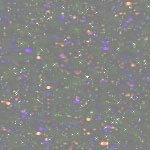
\includegraphics{fix.png}

Long Exposure

Low ISO Speed
\end{center}
\vspace{0.5cm}

%\newpage
%\item Random Noise

Random noise may be the most common image noise. Random noise appears whenever we are using high ISO
values. ISO has mean is a standard which describes its absolute sensitivity to light. 
Quality of camera is good when it remove random noise through software. Example: Neat Image and Noise Ninja programs, they can be removing noise and protect image information. When technology continues to
improve, we can shoot in low light situation.

\begin{center}
	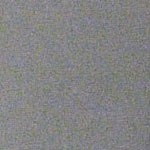
\includegraphics{random.png}

Short Exposure

High ISO Speed
\end{center}



%\item Banding Noise

Banding noise is dependent on what type of camera we are using. With high end cameras, we have never seen banding noise. Banding noise will appear when lower quality photograph are shot with higher
ISO value.
There are causes help banding noise appear: in the dark of photos or increase exposure too much and
digitally make a photograph too bright. We may also see more banding noise in certain white balances which is the process of removing unreal color.
\vspace{0.5cm}

\begin{center}
	
\includegraphics{banding.png}

Susceptible Camera

Brightened Shadows
\end{center}

%\end{itemize}

\subsection*{Denoise}

Noise removal is very important task in image processing. It will help to remove the noise from the image and rebuild to original image is the best quality. In modern digital image processing, data denoising is a hard problem and it used to application areas. Noise removal is popular solution for photography or improve the image was degraded.

\

Filtering is technique which can be decreasing or increasing an image.It's processed value for current pixel will depends itself and surrounding pixels . The value of any pixel in the output image is used by applying  algorithms to the values of the pixels in the place which corresponding input pixel.

\

%Follow Image Processing, there are 4 types of filtering :

%\begin{itemize}
%\item Median Filter.

%The median filter method is very popular in image processing and it protects edges while removing noise in certain environment
%\item Average Filter.

%Average filtering is simply to replace each pixel value in an image with the average value of its area, including itself. Its meaning is remove pixel values which aren't types of their environment.

%\item Gaussian Filter.

%Gaussian filters never go through to function input while minimizing the time.

 
%\item Wiener Filter

%The Wiener filter decreases the mean square error between the random process and the desired process.


%\end{itemize} 
%\end{itemize}

%\vspace*{1cm}











\section{Report organization}
In this report, we have 5 chapters as below :
\begin{itemize}
\item Chapter 1 : Introduction

This chapter included presentation of: Context and Problematic. Context is the part that describe about problems and solutions through this report. Problematic is determination and analysis to problem in this topic. 
\item  Chapter 2 : State Of The Art

Collected different papers addressing the same topics of internship. Next to explain the work published, by giving the context of the work, the main idea, the main results. From this, we can learn more about how to present and solve problems of the authors. 

\item  Chapter 3 : Contribution

In this part, proposed method to solve the problem in the introduction chapter. Beside this, explain method/algorithm/system in proposition.

\item  Chapter 4 \& 5 : Result \& Conclusion

This part include the result of the method/algoritm/system developed. Moreover, it contain comparisons table,  figures, graphics and comment. Recall the problematic, methods used,  contribution, results obtained and future developed.

\end{itemize}






% ----------------------- CHAPITRE ---------------------------

\chapter{State of the art}
\section{Noise Removal in Image Processing using Median [2]}

This paper was written by Monika Kohli and Harmeet Kaur. Authors research and analyze median filter. From this, the filter is compared with median and Adaptive median filter. 
\vspace{1cm}

\textbf{Types of noise}
\vspace{0.5cm}

\textbf{Impulse noise (Salt \& pepper noise):}  Used for this type of noise  Black and white dots appear in this noise so the name salt \& pepper noise. 

\

\textbf{Amplifier noise (Gaussian noise):} 
is the sum of the actual pixel value and a random 

\

\textbf{Quantization noise (Uniform noise):} It appears because quantization process the pixels to a number of discrete levels

\

\textbf{Multiplicative noise (Speckle noise):} It appears because random value multiplications with pixel values of the image as modeled process.



\

\textbf{Periodic noise(Stationary noise):}It appears because attend between electronic components and appear from interference during image acquisition.
%\end{itemize}
\vspace{0.5cm}

After image noise can be classified as above, characteristics of each type are specified. They analyse algorithm of filters : Median filter, Adaptive median filter, Proposed Median Filter.  
\vspace{1cm}

%\textbf{Conclusion}

Finally, Comparison of filters when used PSNR to calculate quality of images with 3 methods : Median filter, Adaptive median filter, Proposed Median Filter. They obtained result show that the proposed method is the best. In future, result can be improved by different noise such as : Gaussian noise, Speckle noise etc
\vspace{2cm}

\section{The Sure-Let Approach to Image Denoising [3]}

 [Thierry Blu \& Florian Luisier]
\vspace{0.5cm}

It’s a new approach to noise removal by the image-domain minimization of an estimate of the mean squared error(MSE). They called  Stein’s unbiased risk estimate (SURE).  They called  Linear expansion of thresholds  (LET) by combination of elementary denoising processes.  Evaluate this denoising performances by comparing PSNR. Combined 3 step above to  SURE-LET Approach.
\vspace{1cm}

%We have SURE-LET Formula as below :
%\begin{center}


%\vspace{0.5cm}
%$\displaystyle\sum_{l=1}^{K}\underbrace{F_k(y)^T F_l(y)a_l}_{[M]_{k,l}} = \underbrace{F_k(y)^Ty-\sigma^2div\left\{F_k(y)\right\}}_{[c]_k}$     
%\vspace{0.2cm}

%$$\hspace{3.5cm} for \ k = 1,2...K$$	
%\end{center}
%\begin{center}
%\hspace{3.5cm} 	$\vspace{0.3cm}\Updownarrow$ 
	

%\hspace{3.5cm}	\textbf{Ma=c} 
%\end{center}

\textbf{Result:}

\

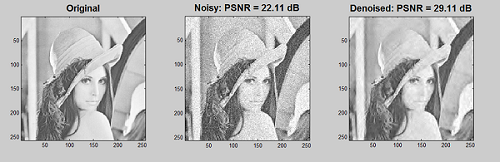
\includegraphics{surelet1.png}

\vspace{1cm}

%\textbf{Conclude:}

Follow SURE-LET program in Matlab, input MSE is compare between noisy image and original image, output MSE is compare between denoise image and original image. So they use output MSE result to table of Comparison Of The Results.
\vspace{1.5cm}

\section{Study on Methods of Noise Reduction in a Stripped Image [4]}

[Chi Chang-yan, Zhang Ji-xian, Liu Zheng-jun]

%\

Noise is one of  image quality problem in the image processing major. Noise reduction is necessary for us to do remove noise and description useful information more prominent. The Gray Value Substitution and Wavelet Transformation are methods in noise removal. Finally, MSE and PSNR are evaluated the processed image suitable in this paper.


%\subsection*{Low pass filter}
%\begin{center}
%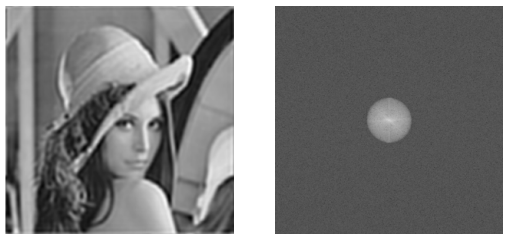
\includegraphics{lowpass.png}


%TLPF processed image and its Fourier spectrum 
%\end{center}
%Noise is high frequency signal, so they used  low pass filter to reduce it. The trapezium low pass filter (TLPF) they choose has certain advantage to smooth transition band. After processing, the image is blur than that before. Low pass filter can remove noise is meaning detailed image information is also removed. So it is not good at image which needs much spectral information. 

%\subsection*{Gray Value Substitution }
\begin{center}
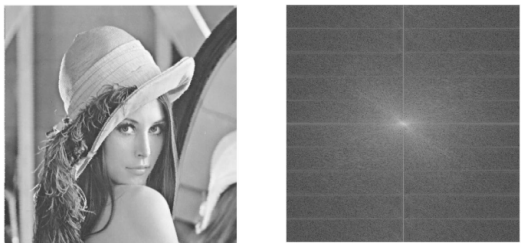
\includegraphics{gray.png}

 Image processing results of gray value substition 
\end{center}

We can see from this image, most noise line is changed and it is not affected by this method.  However, some small noise still appear, and the brightness after processing is stronger than that before. 
\vspace{2cm}
%\subsection*{Wavelet transformation }

\begin{center}
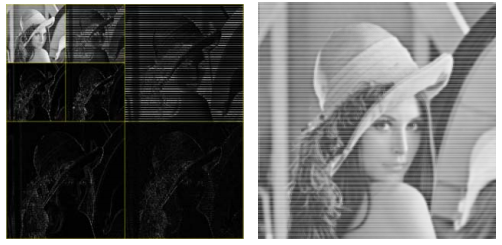
\includegraphics{wave.png}

Image decomposition using Wavelet and usual wavelet denoising result
\end{center}
Wavelet method  haven't solution remove noise in the horizontal domain, the vertical and cross part of image. Moreover this image haven't much noise so they obtain result as above. 

\
%\subsection*{Results and comparisons }

From result tables, they can see that, low pass filter can't use to remove noise. And the other two methods is relatively accepted
\vspace{1.5cm}

\section{Different Noise Types and Digital Image Processing[5]}
[Gursharan Kaur, Rakesh Kumar, Kamaljeet Kainth]


As know, image is used in various fields like medical and education. Noise appear everywhere including images. From this, noise reduction is the main focus to retain the quality of the image.This paper is review problem to types of noise and solution.

\

Types of noise: Gaussian noise, Salt and pepper noise, Poisson noise

\

Different types of linear and non-linear filters.

\

Mean Filter: Mean filter is a type of linear filter that computes average value of the corrupted image.

\

Median Filter: Median filter is a type of non-linear filter. It used to reduce the measure of intensity variation between one pixel and the other pixel.

\

%\subsection*{CONCLUSION AND FUTURE SCOPE}
 In this paper, the purpose is denoising of the images. Techniques that are already using may not be able to find the best result so in the future they may find the techniques that provide optimum solution to the noise.
\vspace{1.5cm}

\section{Impulse Noise Reduction
methods in Digital images [6]}
[Himani Goel, Seema Rani]

\

They review this paper about denoise. From this, compare results by PSNR and MSE to obtain best result. 

\

Linear Filters: Mean filter, Wiener filter.

\

Non Linear filters: Adaptive median
filter, Improved progressive
switching median
filter.

\

%\subsection*{Conclusion}

By the results, they see the median filtering is better than mean or average filter to remove impulse noise but it affect the edge details.
\vspace{1.5cm}

\section{Optimal Gaussian Filter for Effective Noise Filtering [7]}
[Sunil Kopparapu and M Satish]
\vspace{0.5cm}

Noise removal is important problem in many signal processing applications. In this paper, they have show the optimal Gaussian filter that best filters noise, with the noise is AWGN. The contribution of this paper is identification of a method to obtain the optimal Gaussian filter which best filters a signal contaminated with AWGN. 

Gaussian Approach

\

There are basic two ways of remove noise in the signal: 

\

Pre-processing of the signal to enable noise removal  

\

Use of a set of robust algorithms that can compensate for the inherent noise. 

\

In signal processing, pre-processing of the signal is the preferred approach.

\

%\subsection*{Conclusion}
They have shown that the method works well for signals whose bandwidth and the input signal . We are in the process of verifying the validity of their approach for practical signals and finish in the next time.

\section{Image Enhancement with Noise Reduction in Spatial Domain[8]}
[S. Shyam Prasad, R. Priya] 

\



Digital images are mostly corrupted by mixed noise from several sources. It is a big problem have long existed. Generally, some filters can reduce additive or impulse noise, but it can't remove impulsive noise and additive noise. This paper propose change mutual filtering method, which can remove both impulsive and additive noise, when compared to average filter and median filter.  The solve show that the proposed  filtering action can remove impulsive and additive noise while protecting edge.

MODELING NOISE OF THE IMAGES

\

Additive Noise:

\

Additive noise is noise of an image sensor. It's meaning the constant noise in dark areas of the image.

\

Impulse Noise:

\

Impulse noise is called Salt and pepper noise or spike noise. 

\

Mixed Noise:

\

Mixed noise is the combination of additive noise and impulse noise.

\

REMOVING NOISE FROM IMAGES BY FILTERING

\

Linear Filter

Average filter is one of the linear filter.

\

Non-Linear Filters

Median filter and Bilateral filter are the non linear filters.

\

PROPOSED APPROACH

\

Average Filter

The idea of average filtering is simply to replace each pixel value in an image with the average value of its area, including itself.

\  

Median Filter

The median filter is popular technique nonlinear in digital filtering.It removes noise from an image or signal (speckle noise \& salt-pepper noise).


\ 

Bilateral Filter

This is a non-linear technique which can blur an image while taking strong edges. Solve to by combine nonlinear means  with nearby image values. 

\vspace{0.1cm}

\begin{center}
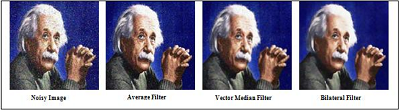
\includegraphics{10.png}

 Quality Measures of Einstein image
\end{center}

 Bilateral filtering method is changed in this paper. It can removed 2 types of noise : impulsive noise and additive noise.


% ----------------------- CHAPITRE ---------------------------

\chapter{Contribution}
Spatial filtering is a types of finite impulse response (FIR) filtering. It is a mask of weights with shape as rectangular. It mean that sliding the mask along the image and apply to multiplication and collection operation on the pixels protected by the mask. 

\section*{Original Image }
First, we are going to read and show original image as below :
%\begin{lstlisting}
%I = imread('lena.tif');
%F = imshow(I);
%\end{lstlisting}

%\textbf{Result:}
\begin{center}
	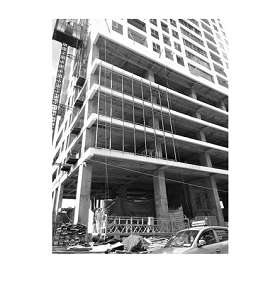
\includegraphics{construction.png}

 Original Image

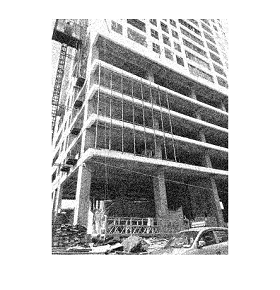
\includegraphics{noisec.png}

Add noise (gaussian noise \& 0.05 variance.)





\end{center}

\section{Median Filter}
Median Filter is family of order filters. It has process : Replace the value of a pixel with the median value of the neighborhood.

$I_{median} = median(I[i,j])$  with $(i,j)\in neighborhood$
\vspace{2cm}
\begin{center}
	

\begin{tabular}{|c|c|c|}  
	\hline 
	30 & 10 & 20 \\ 
	\hline                    
	10 & 250 & 25 \\ 
	\hline 
	20 & 25 & 30 \\ 
	\hline 
\end{tabular} 
\end{center}
\

\



$\Rightarrow$ 10 10 20 20 \textbf{25} 25 30 30 250 

\hspace{26mm}$\uparrow$

\hspace{20mm} median

\newpage
\textbf{Result:}
\vspace{2cm}

\begin{center}
	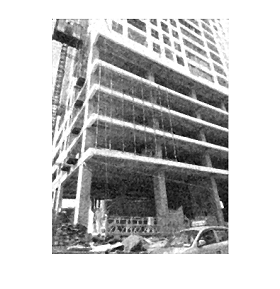
\includegraphics{medianc3.png}
	
	Filter 3$\times$3
\end{center}

\begin{center}
	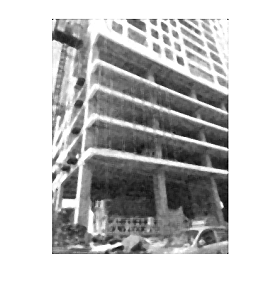
\includegraphics{medianc5.png}

	Filter 5$\times$5
\end{center}
\newpage


\begin{center}
	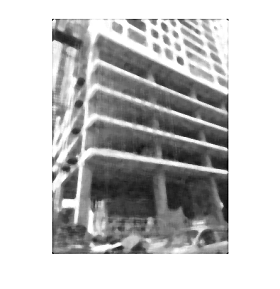
\includegraphics{medianc7.png}
	
		Filter 7$\times$7
\end{center}
\section{Average Filter}

\

Feature: 

Average Filter is spatial filter that applies to a neighborhood (local method). It's a linear filter as a convolution. This mean a pixel is replaced by the average of itself and its neighbours which size determines the amount of smoothing. And equivalent to a filtering operation lowpass.


\

Average Filter have: 
\begin{center}
	Filter 3$\times$3

$\dfrac{1}{9}\begin{tabular}{|c|c|c|}
\hline 
1 & 1 & 1 \\ 
\hline 
1 & 1 & 1 \\ 
\hline 
1 & 1 & 1 \\ 
\hline 
\end{tabular}$ 	
\end{center}

\

\begin{center}
		Filter 5$\times$5
	
	$\dfrac{1}{25}\begin{tabular}{|c|c|c|c|c|}
		\hline 
		1 & 1 & 1 & 1 & 1 \\ 
		\hline 
		1 & 1 & 1 & 1 & 1 \\ 
		\hline 
		1 & 1 & 1 & 1 & 1 \\ 
		\hline 
		1 & 1 & 1 & 1 & 1 \\ 
		\hline 
		1 & 1 & 1 & 1 & 1 \\ 
		\hline 
	\end{tabular} $
\end{center}

\

\begin{center}
	Filter 7$\times$7

$\dfrac{1}{49}\begin{tabular}{|c|c|c|c|c|c|c|}
	\hline 
	1 & 1 & 1 & 1 & 1 & 1 & 1 \\ 
	\hline 
	1 & 1 & 1 & 1 & 1 & 1 & 1 \\ 
	\hline 
	1 & 1 & 1 & 1 & 1 & 1 & 1 \\ 
	\hline 
	1 & 1 & 1 & 1 & 1 & 1 & 1 \\ 
	\hline 
	1 & 1 & 1 & 1 & 1 & 1 & 1 \\ 
	\hline 
	1 & 1 & 1 & 1 & 1 & 1 & 1 \\ 
	\hline 
	1 & 1 & 1 & 1 & 1 & 1 & 1 \\ 
	\hline 
\end{tabular} $
\end{center}
\vspace{1cm}


\textbf{Result:}

\begin{center}
	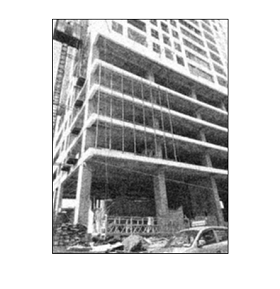
\includegraphics{avec3.png}
	
	Filter $3\times3$
	
	 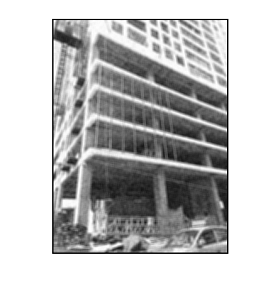
\includegraphics{avec5.png}
	
	Filter $5\times5$
	
		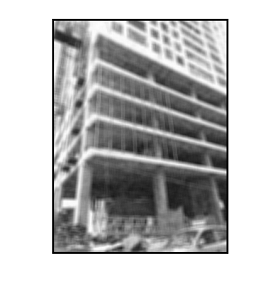
\includegraphics{avec7.png}
	
Filter $7\times7$
\end{center}

\section{Gaussian Filter}

The Gaussian kernel in dimension 2:
\vspace{0.5cm}

$G(x,y) = \dfrac{1}{2\pi\sigma^2}\exp\left[-\dfrac{(x-\mu_x)^2+(y-\mu_y)^2}{2\sigma^2}\right ]$

\vspace{0.5cm}

Define the Gaussian mask($\sigma = 2$):
\vspace{1cm}
%$$\mu = 0$$
%$$
\begin{center}
	Filter 3$\times$3

$\dfrac{1}{16}\begin{tabular}{|c|c|c|}
	\hline 
	1 & 2 & 1 \\ 
	\hline 
	2 & 4 & 2 \\ 
	\hline 
	1 & 2 & 1 \\ 
	\hline 
\end{tabular} $
\end{center}

\begin{center}
	Filter 5$\times$5

$\dfrac{1}{273}\begin{tabular}{|c|c|c|c|c|}
	\hline 
	1 & 4 & 7 & 4 & 1 \\ 
	\hline 
	4 & 16 & 26 & 16 & 4 \\ 
	\hline 
	7 & 26 & 41 & 26 & 7 \\ 
	\hline 
	4 & 16 & 26 & 16 & 4 \\ 
	\hline 
	1 & 4 & 7 & 4 & 1 \\ 
	\hline 
\end{tabular}$ 
\end{center}

\begin{center}
	Filter 7$\times$7

$\dfrac{1}{1003}$\begin{tabular}{|c|c|c|c|c|c|c|}
	\hline 
	0 & 0 & 1 & 2 & 1 & 0 & 0 \\ 
	\hline 
	0 & 3 & 13 & 22 & 13 & 3 & 0 \\ 
	\hline 
	1 & 13 & 59 & 97 & 59 & 13 & 1 \\ 
	\hline 
	2 & 22 & 97 & 159 & 97 & 22 & 2 \\ 
	\hline 
	1 & 13 & 59 & 97 & 59 & 13 & 1 \\ 
	\hline 
	0 & 3 & 13 & 22 & 13 & 3 & 0 \\ 
	\hline 
	0 & 0 & 1 & 2 & 1 & 0 & 0 \\ 
	\hline 
\end{tabular} 
\end{center}
\vspace{1cm}

From theory above, we are going to build function for gaussian filter :
\newpage
\textbf{Result:}

\begin{center}
	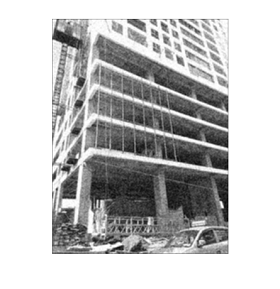
\includegraphics{gauc3.png}
	
	Filter $3\times3$
	
	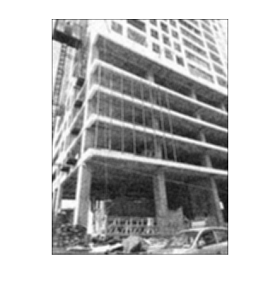
\includegraphics{gauc5.png}
	
	Filter $5\times5$
	
	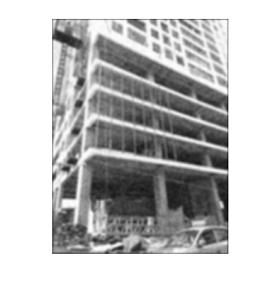
\includegraphics{gauc7.png}
	
	Filter $7\times7$
\end{center}

\section{Wiener Filter}


\textbf{Result:}
\vspace{1cm}
\begin{center}
\includegraphics{Wienec3.png}

Filter $3\times3$

\includegraphics{Wienec5.png}

Filter $5\times5$

\includegraphics{Wienec7.png}

Filter $7\times7$

\end{center}








% ----------------------- CHAPITRE ---------------------------

\chapter{Results}
\section*{Mean Square Error}
In statistics, the mean squared error (MSE) is used to calculate the average of the squares of the errors. It
mean that the difference between the estimator and what is estimated.
The MSE is one of quality evaluation method. In this internship, it help us to know best result when it is the smallest.
 





\

\begin{center}

	$MSE =  \dfrac{1}{n} \displaystyle \sum_{i=1}^{n}(\hat{Y_i} - Y_i)^2$
	

\end{center}
\vspace{3cm}

\section*{Peak signal to noise ratio}
The PSNR is also one of quality evaluation method. In this internship, it help us to know best result when it is the biggest. 

\vspace{1cm}

\begin{center}
	
	$PSNR = 10\log_{10}\left(\dfrac{255^2}{MSE}\right)  $
	
	
\end{center}
\newpage


\section*{Construction Image}
\begin{center}
\begin{figure}[h]
        \begin{subfigure}[b]{0.18\textwidth}
                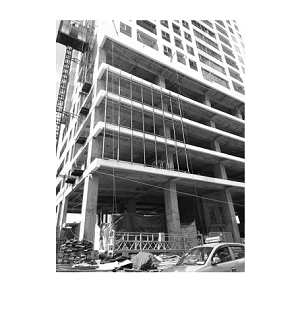
\includegraphics[width=\linewidth]{construction-1.png}
                \caption{Original 1}
                \label{fig:original 1}
        \end{subfigure}%
        \begin{subfigure}[b]{0.18\textwidth}
                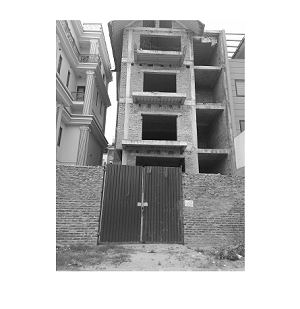
\includegraphics[width=\linewidth]{construction2.png}
                \caption{Original 2}
                \label{fig:original 2}
        \end{subfigure}%
        \begin{subfigure}[b]{0.18\textwidth}
                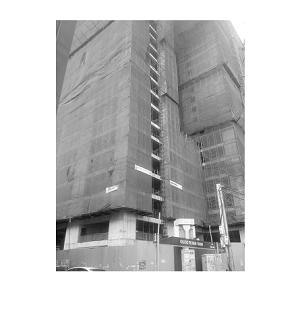
\includegraphics[width=\linewidth]{construction3.png}
                 \caption{Original 3}
                  \label{fig:original 3}
        \end{subfigure}%
        \begin{subfigure}[b]{0.18\textwidth}
                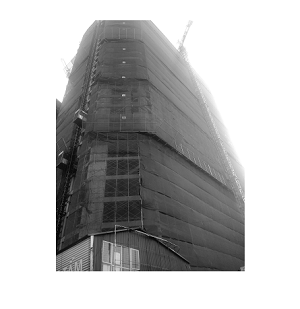
\includegraphics[width=\linewidth]{construction4.png}
                 \caption{Original 4}
                  \label{fig:original 4}
        \end{subfigure}
        \begin{subfigure}[b]{0.18\textwidth}
                        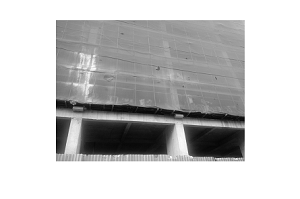
\includegraphics[width=\linewidth]{construction5.png}
                         \caption{Original 5}
                          \label{fig:original 5}
                \end{subfigure}
      \end{figure}
	
\end{center}
\vspace{2cm}

%begin{table}[]
%\centering
%\caption{My caption}
\begin{center}
\begin{tabular}{llllllllllll|l|l|l|l|l|l|l|l|l|l|l|l|l|}
\cline{13-25}
           &            &            &            &            &            &          &          &       &      &      &     & \multicolumn{3}{l|}{Median}  & \multicolumn{3}{l|}{Average} & \multicolumn{4}{l|}{Gaussian} & \multicolumn{3}{l|}{Wiener}           \\ \hline
\multicolumn{4}{|l|}{\multirow{4}{*}{Original 1}} & \multicolumn{4}{l|}{\multirow{2}{*}{Noise}}   & \multicolumn{4}{l|}{MSE}  & \multicolumn{3}{l|}{0.0125}  & \multicolumn{3}{l|}{0.0251}  & \multicolumn{4}{l|}{0.012}    & \multicolumn{3}{l|}{0.0084}           \\ \cline{9-25} 
\multicolumn{4}{|l|}{}                            & \multicolumn{4}{l|}{}                         & \multicolumn{4}{l|}{PSNR} & \multicolumn{3}{l|}{67.1535} & \multicolumn{3}{l|}{64.1264} & \multicolumn{4}{l|}{67.3409}  & \multicolumn{3}{l|}{68.8738}          \\ \cline{5-25} 
\multicolumn{4}{|l|}{}                            & \multicolumn{4}{l|}{\multirow{2}{*}{Denoise}} & \multicolumn{4}{l|}{MSE}  & \multicolumn{3}{l|}{0.0097}  & \multicolumn{3}{l|}{0.022}   & \multicolumn{4}{l|}{0.0095}   & \multicolumn{3}{l|}{\textbf{0.007}}   \\ \cline{9-25} 
\multicolumn{4}{|l|}{}                            & \multicolumn{4}{l|}{}                         & \multicolumn{4}{l|}{PSNR} & \multicolumn{3}{l|}{68.269}  & \multicolumn{3}{l|}{64.7115} & \multicolumn{4}{l|}{68.3762}  & \multicolumn{3}{l|}{\textbf{69.6511}} \\ \hline
\multicolumn{4}{|l|}{\multirow{4}{*}{Original 2}} & \multicolumn{4}{l|}{\multirow{2}{*}{Noise}}   & \multicolumn{4}{l|}{MSE}  & \multicolumn{3}{l|}{0.0096}  & \multicolumn{3}{l|}{0.0219}  & \multicolumn{4}{l|}{0.0096}   & \multicolumn{3}{l|}{0.0075}           \\ \cline{9-25} 
\multicolumn{4}{|l|}{}                            & \multicolumn{4}{l|}{}                         & \multicolumn{4}{l|}{PSNR} & \multicolumn{3}{l|}{68.298}  & \multicolumn{3}{l|}{64.7271} & \multicolumn{4}{l|}{68.2967}  & \multicolumn{3}{l|}{69.3898}          \\ \cline{5-25} 
\multicolumn{4}{|l|}{}                            & \multicolumn{4}{l|}{\multirow{2}{*}{Denoise}} & \multicolumn{4}{l|}{MSE}  & \multicolumn{3}{l|}{0.0055}  & \multicolumn{3}{l|}{0.0166}  & \multicolumn{4}{l|}{0.0056}   & \multicolumn{3}{l|}{\textbf{0.0044}}  \\ \cline{9-25} 
\multicolumn{4}{|l|}{}                            & \multicolumn{4}{l|}{}                         & \multicolumn{4}{l|}{PSNR} & \multicolumn{3}{l|}{70.7071} & \multicolumn{3}{l|}{65.9348} & \multicolumn{4}{l|}{70.6237}  & \multicolumn{3}{l|}{\textbf{71.654}}  \\ \hline
\multicolumn{4}{|l|}{\multirow{4}{*}{Original 3}} & \multicolumn{4}{l|}{\multirow{2}{*}{Noise}}   & \multicolumn{4}{l|}{MSE}  & \multicolumn{3}{l|}{0.0078}  & \multicolumn{3}{l|}{0.0178}  & \multicolumn{4}{l|}{0.0077}   & \multicolumn{3}{l|}{0.0061}           \\ \cline{9-25} 
\multicolumn{4}{|l|}{}                            & \multicolumn{4}{l|}{}                         & \multicolumn{4}{l|}{PSNR} & \multicolumn{3}{l|}{69.2093} & \multicolumn{3}{l|}{65.638}  & \multicolumn{4}{l|}{69.2572}  & \multicolumn{3}{l|}{70.2559}          \\ \cline{5-25} 
\multicolumn{4}{|l|}{}                            & \multicolumn{4}{l|}{\multirow{2}{*}{Denoise}} & \multicolumn{4}{l|}{MSE}  & \multicolumn{3}{l|}{0.0034}  & \multicolumn{3}{l|}{0.0122}  & \multicolumn{4}{l|}{0.0035}   & \multicolumn{3}{l|}{\textbf{0.0028}}  \\ \cline{9-25} 
\multicolumn{4}{|l|}{}                            & \multicolumn{4}{l|}{}                         & \multicolumn{4}{l|}{PSNR} & \multicolumn{3}{l|}{72.761}  & \multicolumn{3}{l|}{67.2713} & \multicolumn{4}{l|}{72.6781}  & \multicolumn{3}{l|}{\textbf{73.6324}} \\ \hline
\multicolumn{4}{|l|}{\multirow{4}{*}{Original 4}} & \multicolumn{4}{l|}{\multirow{2}{*}{Noise}}   & \multicolumn{4}{l|}{MSE}  & \multicolumn{3}{l|}{0.0065}  & \multicolumn{3}{l|}{0.0183}  & \multicolumn{4}{l|}{0.0067}   & \multicolumn{3}{l|}{0.0054}           \\ \cline{9-25} 
\multicolumn{4}{|l|}{}                            & \multicolumn{4}{l|}{}                         & \multicolumn{4}{l|}{PSNR} & \multicolumn{3}{l|}{69.9904} & \multicolumn{3}{l|}{65.5003} & \multicolumn{4}{l|}{69.8929}  & \multicolumn{3}{l|}{70.8107}          \\ \cline{5-25} 
\multicolumn{4}{|l|}{}                            & \multicolumn{4}{l|}{\multirow{2}{*}{Denoise}} & \multicolumn{4}{l|}{MSE}  & \multicolumn{3}{l|}{0.0026}  & \multicolumn{3}{l|}{0.0144}  & \multicolumn{4}{l|}{0.0031}   & \multicolumn{3}{l|}{\textbf{0.0022}}  \\ \cline{9-25} 
\multicolumn{4}{|l|}{}                            & \multicolumn{4}{l|}{}                         & \multicolumn{4}{l|}{PSNR} & \multicolumn{3}{l|}{73.9221} & \multicolumn{3}{l|}{66.5571} & \multicolumn{4}{l|}{73.1714}  & \multicolumn{3}{l|}{\textbf{74.65}}   \\ \hline
\multicolumn{4}{|l|}{\multirow{4}{*}{Original 5}} & \multicolumn{4}{l|}{\multirow{2}{*}{Noise}}   & \multicolumn{4}{l|}{MSE}  & \multicolumn{3}{l|}{0.0125}  & \multicolumn{3}{l|}{0.0351}  & \multicolumn{4}{l|}{0.0131}   & \multicolumn{3}{l|}{0.0098}           \\ \cline{9-25} 
\multicolumn{4}{|l|}{}                            & \multicolumn{4}{l|}{}                         & \multicolumn{4}{l|}{PSNR} & \multicolumn{3}{l|}{67.1789} & \multicolumn{3}{l|}{62.6729} & \multicolumn{4}{l|}{66.9615}  & \multicolumn{3}{l|}{68.2047}          \\ \cline{5-25} 
\multicolumn{4}{|l|}{}                            & \multicolumn{4}{l|}{\multirow{2}{*}{Denoise}} & \multicolumn{4}{l|}{MSE}  & \multicolumn{3}{l|}{0.0048}  & \multicolumn{3}{l|}{0.0243}  & \multicolumn{4}{l|}{0.0056}   & \multicolumn{3}{l|}{\textbf{0.0046}}  \\ \cline{9-25} 
\multicolumn{4}{|l|}{}                            & \multicolumn{4}{l|}{}                         & \multicolumn{4}{l|}{PSNR} & \multicolumn{3}{l|}{71.3083} & \multicolumn{3}{l|}{64.2764} & \multicolumn{4}{l|}{70.6356}  & \multicolumn{3}{l|}{\textbf{71.5275}} \\ \hline
\end{tabular}

\

Comparison Table
\end{center}










\newpage
\section*{Rubbish Image}
\begin{center}
\begin{figure}[h]
        \begin{subfigure}[b]{0.18\textwidth}
                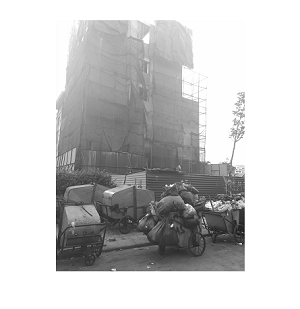
\includegraphics[width=\linewidth]{rubbish1.png}
                \caption{Original 1}
                \label{fig:original 1}
        \end{subfigure}%
        \begin{subfigure}[b]{0.18\textwidth}
                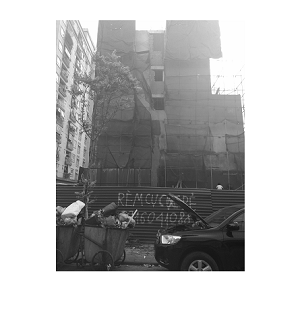
\includegraphics[width=\linewidth]{rubbish2.png}
                \caption{Original 2}
                \label{fig:original 2}
        \end{subfigure}%
        \begin{subfigure}[b]{0.18\textwidth}
                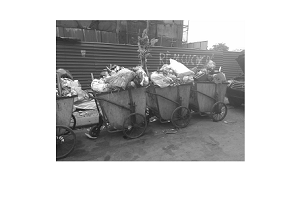
\includegraphics[width=\linewidth]{rubbish3.png}
                 \caption{Original 3}
                  \label{fig:original 3}
        \end{subfigure}%
        \begin{subfigure}[b]{0.18\textwidth}
                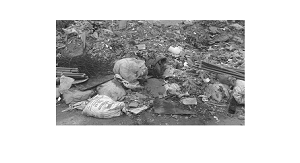
\includegraphics[width=\linewidth]{rubbish4.png}
                 \caption{Original 4}
                  \label{fig:original 4}
        \end{subfigure}
        \begin{subfigure}[b]{0.18\textwidth}
                        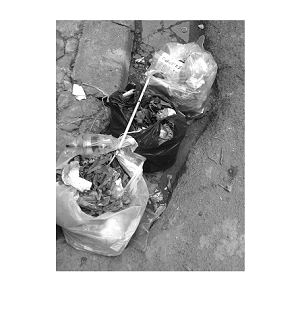
\includegraphics[width=\linewidth]{rubbish5.png}
                         \caption{Original 5}
                          \label{fig:original 5}
                \end{subfigure}
      \end{figure}
	\end{center}
\vspace{2cm}

\begin{center}


\begin{tabular}{llllllllllll|l|l|l|l|l|l|l|l|l|l|l|l|l|}
\cline{13-25}
           &            &            &            &            &            &          &          &       &      &      &     & \multicolumn{3}{l|}{Median}  & \multicolumn{3}{l|}{Average}          & \multicolumn{4}{l|}{Gaussian} & \multicolumn{3}{l|}{Wiener}           \\ \hline
\multicolumn{4}{|l|}{\multirow{4}{*}{Original 1}} & \multicolumn{4}{l|}{\multirow{2}{*}{Noise}}   & \multicolumn{4}{l|}{MSE}  & \multicolumn{3}{l|}{0.007}   & \multicolumn{3}{l|}{0.0198}           & \multicolumn{4}{l|}{0.007}    & \multicolumn{3}{l|}{0.0053}           \\ \cline{9-25} 
\multicolumn{4}{|l|}{}                            & \multicolumn{4}{l|}{}                         & \multicolumn{4}{l|}{PSNR} & \multicolumn{3}{l|}{69.6741} & \multicolumn{3}{l|}{65.1589}          & \multicolumn{4}{l|}{69.6536}  & \multicolumn{3}{l|}{70.8804}          \\ \cline{5-25} 
\multicolumn{4}{|l|}{}                            & \multicolumn{4}{l|}{\multirow{2}{*}{Denoise}} & \multicolumn{4}{l|}{MSE}  & \multicolumn{3}{l|}{0.0032}  & \multicolumn{3}{l|}{0.0156}           & \multicolumn{4}{l|}{0.0036}   & \multicolumn{3}{l|}{\textbf{0.0025}}  \\ \cline{9-25} 
\multicolumn{4}{|l|}{}                            & \multicolumn{4}{l|}{}                         & \multicolumn{4}{l|}{PSNR} & \multicolumn{3}{l|}{73.1106} & \multicolumn{3}{l|}{66.1969}          & \multicolumn{4}{l|}{72.5825}  & \multicolumn{3}{l|}{\textbf{74.1694}} \\ \hline
\multicolumn{4}{|l|}{\multirow{4}{*}{Original 2}} & \multicolumn{4}{l|}{\multirow{2}{*}{Noise}}   & \multicolumn{4}{l|}{MSE}  & \multicolumn{3}{l|}{0.0078}  & \multicolumn{3}{l|}{0.0173}           & \multicolumn{4}{l|}{0.0076}   & \multicolumn{3}{l|}{0.0061}           \\ \cline{9-25} 
\multicolumn{4}{|l|}{}                            & \multicolumn{4}{l|}{}                         & \multicolumn{4}{l|}{PSNR} & \multicolumn{3}{l|}{69.2119} & \multicolumn{3}{l|}{65.7582}          & \multicolumn{4}{l|}{69.3064}  & \multicolumn{3}{l|}{70.2561}          \\ \cline{5-25} 
\multicolumn{4}{|l|}{}                            & \multicolumn{4}{l|}{\multirow{2}{*}{Denoise}} & \multicolumn{4}{l|}{MSE}  & \multicolumn{3}{l|}{0.0036}  & \multicolumn{3}{l|}{\textbf{0.00126}} & \multicolumn{4}{l|}{0.0038}   & \multicolumn{3}{l|}{0.0029}           \\ \cline{9-25} 
\multicolumn{4}{|l|}{}                            & \multicolumn{4}{l|}{}                         & \multicolumn{4}{l|}{PSNR} & \multicolumn{3}{l|}{72.5146} & \multicolumn{3}{l|}{67.1263}          & \multicolumn{4}{l|}{72.3851}  & \multicolumn{3}{l|}{\textbf{73.4524}} \\ \hline
\multicolumn{4}{|l|}{\multirow{4}{*}{Original 3}} & \multicolumn{4}{l|}{\multirow{2}{*}{Noise}}   & \multicolumn{4}{l|}{MSE}  & \multicolumn{3}{l|}{0.0158}  & \multicolumn{3}{l|}{0.0336}           & \multicolumn{4}{l|}{0.015}    & \multicolumn{3}{l|}{0.0115}           \\ \cline{9-25} 
\multicolumn{4}{|l|}{}                            & \multicolumn{4}{l|}{}                         & \multicolumn{4}{l|}{PSNR} & \multicolumn{3}{l|}{66.1394} & \multicolumn{3}{l|}{62.8625}          & \multicolumn{4}{l|}{66.3823}  & \multicolumn{3}{l|}{67.5195}          \\ \cline{5-25} 
\multicolumn{4}{|l|}{}                            & \multicolumn{4}{l|}{\multirow{2}{*}{Denoise}} & \multicolumn{4}{l|}{MSE}  & \multicolumn{3}{l|}{0.0083}  & \multicolumn{3}{l|}{0.0246}           & \multicolumn{4}{l|}{0.0081}   & \multicolumn{3}{l|}{\textbf{0.0063}}  \\ \cline{9-25} 
\multicolumn{4}{|l|}{}                            & \multicolumn{4}{l|}{}                         & \multicolumn{4}{l|}{PSNR} & \multicolumn{3}{l|}{68.9656} & \multicolumn{3}{l|}{64.2139}          & \multicolumn{4}{l|}{69.0718}  & \multicolumn{3}{l|}{\textbf{70.1636}} \\ \hline
\multicolumn{4}{|l|}{\multirow{4}{*}{Original 4}} & \multicolumn{4}{l|}{\multirow{2}{*}{Noise}}   & \multicolumn{4}{l|}{MSE}  & \multicolumn{3}{l|}{0.0313}  & \multicolumn{3}{l|}{0.0567}           & \multicolumn{4}{l|}{0.0287}   & \multicolumn{3}{l|}{0.0235}           \\ \cline{9-25} 
\multicolumn{4}{|l|}{}                            & \multicolumn{4}{l|}{}                         & \multicolumn{4}{l|}{PSNR} & \multicolumn{3}{l|}{63.1696} & \multicolumn{3}{l|}{60.5959}          & \multicolumn{4}{l|}{63.5549}  & \multicolumn{3}{l|}{64.4181}          \\ \cline{5-25} 
\multicolumn{4}{|l|}{}                            & \multicolumn{4}{l|}{\multirow{2}{*}{Denoise}} & \multicolumn{4}{l|}{MSE}  & \multicolumn{3}{l|}{0.0207}  & \multicolumn{3}{l|}{0.0424}           & \multicolumn{4}{l|}{0.0185}   & \multicolumn{3}{l|}{\textbf{0.0161}}  \\ \cline{9-25} 
\multicolumn{4}{|l|}{}                            & \multicolumn{4}{l|}{}                         & \multicolumn{4}{l|}{PSNR} & \multicolumn{3}{l|}{64.9661} & \multicolumn{3}{l|}{61.8601}          & \multicolumn{4}{l|}{65.4527}  & \multicolumn{3}{l|}{\textbf{66.0756}} \\ \hline
\multicolumn{4}{|l|}{\multirow{4}{*}{Original 5}} & \multicolumn{4}{l|}{\multirow{2}{*}{Noise}}   & \multicolumn{4}{l|}{MSE}  & \multicolumn{3}{l|}{0.0096}  & \multicolumn{3}{l|}{0.0176}           & \multicolumn{4}{l|}{0.0092}   & \multicolumn{3}{l|}{0.007}            \\ \cline{9-25} 
\multicolumn{4}{|l|}{}                            & \multicolumn{4}{l|}{}                         & \multicolumn{4}{l|}{PSNR} & \multicolumn{3}{l|}{68.3119} & \multicolumn{3}{l|}{65.677}           & \multicolumn{4}{l|}{68.4872}  & \multicolumn{3}{l|}{69.698}           \\ \cline{5-25} 
\multicolumn{4}{|l|}{}                            & \multicolumn{4}{l|}{\multirow{2}{*}{Denoise}} & \multicolumn{4}{l|}{MSE}  & \multicolumn{3}{l|}{0.0055}  & \multicolumn{3}{l|}{0.0123}           & \multicolumn{4}{l|}{0.0053}   & \multicolumn{3}{l|}{\textbf{0.004}}   \\ \cline{9-25} 
\multicolumn{4}{|l|}{}                            & \multicolumn{4}{l|}{}                         & \multicolumn{4}{l|}{PSNR} & \multicolumn{3}{l|}{70.7050} & \multicolumn{3}{l|}{67.2474}          & \multicolumn{4}{l|}{70.9133}  & \multicolumn{3}{l|}{\textbf{72.0813}} \\ \hline
\end{tabular}
	
	\
	
	Comparison Table
\end{center}

\newpage
\section*{Pagoda Image}
\begin{center}
\begin{figure}[h]
        \begin{subfigure}[b]{0.18\textwidth}
                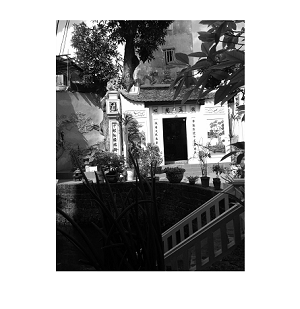
\includegraphics[width=\linewidth]{pagoda1.png}
                \caption{Original 1}
                \label{fig:original 1}
        \end{subfigure}%
        \begin{subfigure}[b]{0.18\textwidth}
                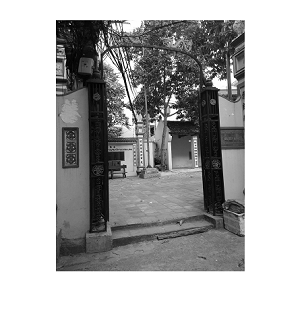
\includegraphics[width=\linewidth]{pagoda2.png}
                \caption{Original 2}
                \label{fig:original 2}
        \end{subfigure}%
        \begin{subfigure}[b]{0.18\textwidth}
                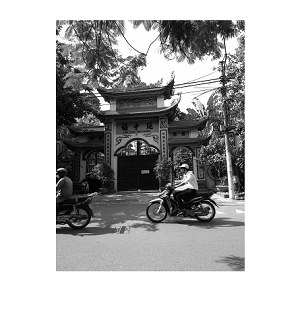
\includegraphics[width=\linewidth]{pagoda3.png}
                 \caption{Original 3}
                  \label{fig:original 3}
        \end{subfigure}%
        \begin{subfigure}[b]{0.18\textwidth}
                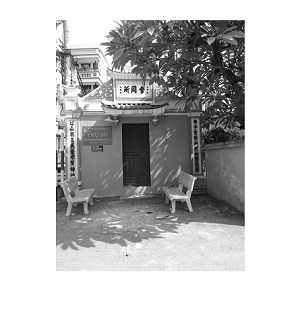
\includegraphics[width=\linewidth]{pagoda4.png}
                 \caption{Original 4}
                  \label{fig:original 4}
        \end{subfigure}
        \begin{subfigure}[b]{0.18\textwidth}
                        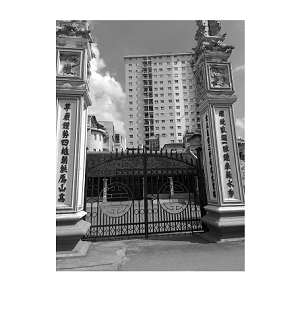
\includegraphics[width=\linewidth]{pagoda5.png}
                         \caption{Original 5}
                          \label{fig:original 5}
                \end{subfigure}
      \end{figure}
\end{center}
\vspace{2cm}

\begin{center}
\begin{tabular}{llllllllllll|l|l|l|l|l|l|l|l|l|l|l|l|l|}
\cline{13-25}
           &            &            &            &            &            &          &          &       &      &      &     & \multicolumn{3}{l|}{Median}  & \multicolumn{3}{l|}{Average} & \multicolumn{4}{l|}{Gaussian} & \multicolumn{3}{l|}{Wiener}           \\ \hline
\multicolumn{4}{|l|}{\multirow{4}{*}{Original 1}} & \multicolumn{4}{l|}{\multirow{2}{*}{Noise}}   & \multicolumn{4}{l|}{MSE}  & \multicolumn{3}{l|}{0.013}   & \multicolumn{3}{l|}{0.0168}  & \multicolumn{4}{l|}{0.0115}   & \multicolumn{3}{l|}{0.0068}           \\ \cline{9-25} 
\multicolumn{4}{|l|}{}                            & \multicolumn{4}{l|}{}                         & \multicolumn{4}{l|}{PSNR} & \multicolumn{3}{l|}{66.9999} & \multicolumn{3}{l|}{65.8739} & \multicolumn{4}{l|}{67.5091}  & \multicolumn{3}{l|}{69.7993}          \\ \cline{5-25} 
\multicolumn{4}{|l|}{}                            & \multicolumn{4}{l|}{\multirow{2}{*}{Denoise}} & \multicolumn{4}{l|}{MSE}  & \multicolumn{3}{l|}{0.0098}  & \multicolumn{3}{l|}{0.0141}  & \multicolumn{4}{l|}{0.0093}   & \multicolumn{3}{l|}{\textbf{0.0055}}  \\ \cline{9-25} 
\multicolumn{4}{|l|}{}                            & \multicolumn{4}{l|}{}                         & \multicolumn{4}{l|}{PSNR} & \multicolumn{3}{l|}{68.2117} & \multicolumn{3}{l|}{66.6490} & \multicolumn{4}{l|}{68.4598}  & \multicolumn{3}{l|}{\textbf{70.7544}} \\ \hline
\multicolumn{4}{|l|}{\multirow{4}{*}{Original 2}} & \multicolumn{4}{l|}{\multirow{2}{*}{Noise}}   & \multicolumn{4}{l|}{MSE}  & \multicolumn{3}{l|}{0.0138}  & \multicolumn{3}{l|}{0.0189}  & \multicolumn{4}{l|}{0.0122}   & \multicolumn{3}{l|}{0.0076}           \\ \cline{9-25} 
\multicolumn{4}{|l|}{}                            & \multicolumn{4}{l|}{}                         & \multicolumn{4}{l|}{PSNR} & \multicolumn{3}{l|}{66.7404} & \multicolumn{3}{l|}{65.3739} & \multicolumn{4}{l|}{67.2818}  & \multicolumn{3}{l|}{69.3011}          \\ \cline{5-25} 
\multicolumn{4}{|l|}{}                            & \multicolumn{4}{l|}{\multirow{2}{*}{Denoise}} & \multicolumn{4}{l|}{MSE}  & \multicolumn{3}{l|}{0.0098}  & \multicolumn{3}{l|}{0.0145}  & \multicolumn{4}{l|}{0.0088}   & \multicolumn{3}{l|}{\textbf{0.0053}}  \\ \cline{9-25} 
\multicolumn{4}{|l|}{}                            & \multicolumn{4}{l|}{}                         & \multicolumn{4}{l|}{PSNR} & \multicolumn{3}{l|}{68.2338} & \multicolumn{3}{l|}{66.5220} & \multicolumn{4}{l|}{68.6970}  & \multicolumn{3}{l|}{\textbf{70.9009}} \\ \hline
\multicolumn{4}{|l|}{\multirow{4}{*}{Original 3}} & \multicolumn{4}{l|}{\multirow{2}{*}{Noise}}   & \multicolumn{4}{l|}{MSE}  & \multicolumn{3}{l|}{0.0150}  & \multicolumn{3}{l|}{0.0215}  & \multicolumn{4}{l|}{0.0131}   & \multicolumn{3}{l|}{0.0081}           \\ \cline{9-25} 
\multicolumn{4}{|l|}{}                            & \multicolumn{4}{l|}{}                         & \multicolumn{4}{l|}{PSNR} & \multicolumn{3}{l|}{66.3743} & \multicolumn{3}{l|}{64.8131} & \multicolumn{4}{l|}{66.9631}  & \multicolumn{3}{l|}{69.0515}          \\ \cline{5-25} 
\multicolumn{4}{|l|}{}                            & \multicolumn{4}{l|}{\multirow{2}{*}{Denoise}} & \multicolumn{4}{l|}{MSE}  & \multicolumn{3}{l|}{0.0114}  & \multicolumn{3}{l|}{0.0177}  & \multicolumn{4}{l|}{0.0102}   & \multicolumn{3}{l|}{\textbf{0.0065}}  \\ \cline{9-25} 
\multicolumn{4}{|l|}{}                            & \multicolumn{4}{l|}{}                         & \multicolumn{4}{l|}{PSNR} & \multicolumn{3}{l|}{67.5543} & \multicolumn{3}{l|}{65.6549} & \multicolumn{4}{l|}{68.0291}  & \multicolumn{3}{l|}{\textbf{70.0034}} \\ \hline
\multicolumn{4}{|l|}{\multirow{4}{*}{Original 4}} & \multicolumn{4}{l|}{\multirow{2}{*}{Noise}}   & \multicolumn{4}{l|}{MSE}  & \multicolumn{3}{l|}{0.0116}  & \multicolumn{3}{l|}{0.0229}  & \multicolumn{4}{l|}{0.0106}   & \multicolumn{3}{l|}{0.0069}           \\ \cline{9-25} 
\multicolumn{4}{|l|}{}                            & \multicolumn{4}{l|}{}                         & \multicolumn{4}{l|}{PSNR} & \multicolumn{3}{l|}{67.4972} & \multicolumn{3}{l|}{64.5418} & \multicolumn{4}{l|}{67.8751}  & \multicolumn{3}{l|}{69.7300}          \\ \cline{5-25} 
\multicolumn{4}{|l|}{}                            & \multicolumn{4}{l|}{\multirow{2}{*}{Denoise}} & \multicolumn{4}{l|}{MSE}  & \multicolumn{3}{l|}{0.0080}  & \multicolumn{3}{l|}{0.0188}  & \multicolumn{4}{l|}{0.0072}   & \multicolumn{3}{l|}{\textbf{0.0047}}  \\ \cline{9-25} 
\multicolumn{4}{|l|}{}                            & \multicolumn{4}{l|}{}                         & \multicolumn{4}{l|}{PSNR} & \multicolumn{3}{l|}{69.1060} & \multicolumn{3}{l|}{65.3952} & \multicolumn{4}{l|}{69.5399}  & \multicolumn{3}{l|}{\textbf{71.4029}} \\ \hline
\multicolumn{4}{|l|}{\multirow{4}{*}{Original 5}} & \multicolumn{4}{l|}{\multirow{2}{*}{Noise}}   & \multicolumn{4}{l|}{MSE}  & \multicolumn{3}{l|}{0.0141}  & \multicolumn{3}{l|}{0.0230}  & \multicolumn{4}{l|}{0.0125}   & \multicolumn{3}{l|}{0.0086}           \\ \cline{9-25} 
\multicolumn{4}{|l|}{}                            & \multicolumn{4}{l|}{}                         & \multicolumn{4}{l|}{PSNR} & \multicolumn{3}{l|}{66.6335} & \multicolumn{3}{l|}{64.5060} & \multicolumn{4}{l|}{67.1643}  & \multicolumn{3}{l|}{68.8033}          \\ \cline{5-25} 
\multicolumn{4}{|l|}{}                            & \multicolumn{4}{l|}{\multirow{2}{*}{Denoise}} & \multicolumn{4}{l|}{MSE}  & \multicolumn{3}{l|}{0.0104}  & \multicolumn{3}{l|}{0.0179}  & \multicolumn{4}{l|}{0.0087}   & \multicolumn{3}{l|}{\textbf{0.0062}}  \\ \cline{9-25} 
\multicolumn{4}{|l|}{}                            & \multicolumn{4}{l|}{}                         & \multicolumn{4}{l|}{PSNR} & \multicolumn{3}{l|}{67.9741} & \multicolumn{3}{l|}{65.6092} & \multicolumn{4}{l|}{68.7310}  & \multicolumn{3}{l|}{\textbf{70.2064}} \\ \hline
\end{tabular}

\

Comparison Table
\end{center}


\newpage
\section*{Pond Image}
\begin{center}
\begin{figure}[h]
        \begin{subfigure}[b]{0.18\textwidth}
                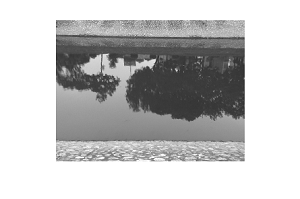
\includegraphics[width=\linewidth]{pond1.png}
                \caption{Original 1}
                \label{fig:original 1}
        \end{subfigure}%
        \begin{subfigure}[b]{0.18\textwidth}
                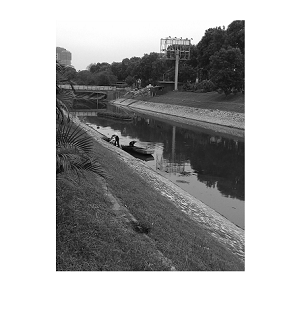
\includegraphics[width=\linewidth]{pond2.png}
                \caption{Original 2}
                \label{fig:original 2}
        \end{subfigure}%
        \begin{subfigure}[b]{0.18\textwidth}
                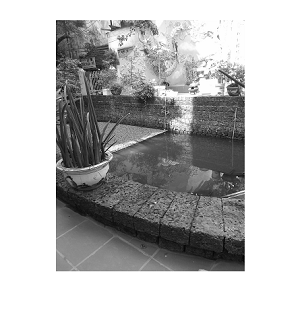
\includegraphics[width=\linewidth]{pond3.png}
                 \caption{Original 3}
                  \label{fig:original 3}
        \end{subfigure}%
        \begin{subfigure}[b]{0.18\textwidth}
                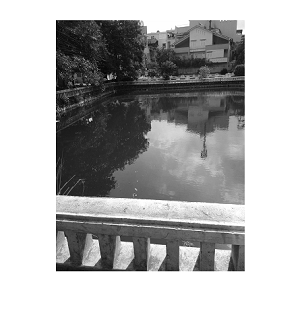
\includegraphics[width=\linewidth]{pond4.png}
                 \caption{Original 4}
                  \label{fig:original 4}
        \end{subfigure}
        \begin{subfigure}[b]{0.18\textwidth}
                        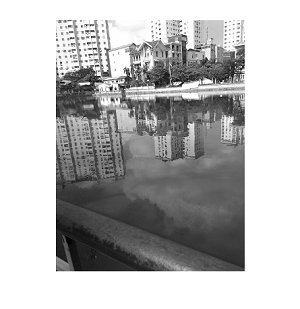
\includegraphics[width=\linewidth]{pond5.png}
                         \caption{Original 5}
                          \label{fig:original 5}
                \end{subfigure}
      \end{figure}
\end{center}
\vspace{2cm}

\begin{center}
\begin{tabular}{llllllllllll|l|l|l|l|l|l|l|l|l|l|l|l|l|}
\cline{13-25}
           &            &            &            &            &            &          &          &       &      &      &     & \multicolumn{3}{l|}{Median}  & \multicolumn{3}{l|}{Average} & \multicolumn{4}{l|}{Gaussian} & \multicolumn{3}{l|}{Wiener}           \\ \hline
\multicolumn{4}{|l|}{\multirow{4}{*}{Original 1}} & \multicolumn{4}{l|}{\multirow{2}{*}{Noise}}   & \multicolumn{4}{l|}{MSE}  & \multicolumn{3}{l|}{0.0151}  & \multicolumn{3}{l|}{0.0374}  & \multicolumn{4}{l|}{0.0148}   & \multicolumn{3}{l|}{0.0116}           \\ \cline{9-25} 
\multicolumn{4}{|l|}{}                            & \multicolumn{4}{l|}{}                         & \multicolumn{4}{l|}{PSNR} & \multicolumn{3}{l|}{66.3488} & \multicolumn{3}{l|}{62.4067} & \multicolumn{4}{l|}{66.4381}  & \multicolumn{3}{l|}{69.5}             \\ \cline{5-25} 
\multicolumn{4}{|l|}{}                            & \multicolumn{4}{l|}{\multirow{2}{*}{Denoise}} & \multicolumn{4}{l|}{MSE}  & \multicolumn{3}{l|}{0.0071}  & \multicolumn{3}{l|}{0.0267}  & \multicolumn{4}{l|}{0.0071}   & \multicolumn{3}{l|}{\textbf{0.0057}}  \\ \cline{9-25} 
\multicolumn{4}{|l|}{}                            & \multicolumn{4}{l|}{}                         & \multicolumn{4}{l|}{PSNR} & \multicolumn{3}{l|}{69.6156} & \multicolumn{3}{l|}{63.8625} & \multicolumn{4}{l|}{69.6193}  & \multicolumn{3}{l|}{\textbf{70.5647}} \\ \hline
\multicolumn{4}{|l|}{\multirow{4}{*}{Original 2}} & \multicolumn{4}{l|}{\multirow{2}{*}{Noise}}   & \multicolumn{4}{l|}{MSE}  & \multicolumn{3}{l|}{0.009}   & \multicolumn{3}{l|}{0.0161}  & \multicolumn{4}{l|}{0.087}    & \multicolumn{3}{l|}{0.0066}           \\ \cline{9-25} 
\multicolumn{4}{|l|}{}                            & \multicolumn{4}{l|}{}                         & \multicolumn{4}{l|}{PSNR} & \multicolumn{3}{l|}{68.5651} & \multicolumn{3}{l|}{66.0539} & \multicolumn{4}{l|}{68.7473}  & \multicolumn{3}{l|}{69.9595}          \\ \cline{5-25} 
\multicolumn{4}{|l|}{}                            & \multicolumn{4}{l|}{\multirow{2}{*}{Denoise}} & \multicolumn{4}{l|}{MSE}  & \multicolumn{3}{l|}{0.0049}  & \multicolumn{3}{l|}{0.0118}  & \multicolumn{4}{l|}{0.0049}   & \multicolumn{3}{l|}{\textbf{0.0037}}  \\ \cline{9-25} 
\multicolumn{4}{|l|}{}                            & \multicolumn{4}{l|}{}                         & \multicolumn{4}{l|}{PSNR} & \multicolumn{3}{l|}{71.1950} & \multicolumn{3}{l|}{67.4075} & \multicolumn{4}{l|}{71.1985}  & \multicolumn{3}{l|}{\textbf{72.4594}} \\ \hline
\multicolumn{4}{|l|}{\multirow{4}{*}{Original 3}} & \multicolumn{4}{l|}{\multirow{2}{*}{Noise}}   & \multicolumn{4}{l|}{MSE}  & \multicolumn{3}{l|}{0.0103}  & \multicolumn{3}{l|}{0.0181}  & \multicolumn{4}{l|}{0.0095}   & \multicolumn{3}{l|}{0.0071}           \\ \cline{9-25} 
\multicolumn{4}{|l|}{}                            & \multicolumn{4}{l|}{}                         & \multicolumn{4}{l|}{PSNR} & \multicolumn{3}{l|}{68.0057} & \multicolumn{3}{l|}{65.5457} & \multicolumn{4}{l|}{68.3309}  & \multicolumn{3}{l|}{69.5910}          \\ \cline{5-25} 
\multicolumn{4}{|l|}{}                            & \multicolumn{4}{l|}{\multirow{2}{*}{Denoise}} & \multicolumn{4}{l|}{MSE}  & \multicolumn{3}{l|}{0.0063}  & \multicolumn{3}{l|}{0.0136}  & \multicolumn{4}{l|}{0.0059}   & \multicolumn{3}{l|}{\textbf{0.0045}}  \\ \cline{9-25} 
\multicolumn{4}{|l|}{}                            & \multicolumn{4}{l|}{}                         & \multicolumn{4}{l|}{PSNR} & \multicolumn{3}{l|}{70.1294} & \multicolumn{3}{l|}{66.7905} & \multicolumn{4}{l|}{70.4278}  & \multicolumn{3}{l|}{\textbf{71.5971}} \\ \hline
\multicolumn{4}{|l|}{\multirow{4}{*}{Original 4}} & \multicolumn{4}{l|}{\multirow{2}{*}{Noise}}   & \multicolumn{4}{l|}{MSE}  & \multicolumn{3}{l|}{0.0085}  & \multicolumn{3}{l|}{0.0148}  & \multicolumn{4}{l|}{0.0082}   & \multicolumn{3}{l|}{0.0062}           \\ \cline{9-25} 
\multicolumn{4}{|l|}{}                            & \multicolumn{4}{l|}{}                         & \multicolumn{4}{l|}{PSNR} & \multicolumn{3}{l|}{68.8176} & \multicolumn{3}{l|}{66.4207} & \multicolumn{4}{l|}{68.9979}  & \multicolumn{3}{l|}{70.1919}          \\ \cline{5-25} 
\multicolumn{4}{|l|}{}                            & \multicolumn{4}{l|}{\multirow{2}{*}{Denoise}} & \multicolumn{4}{l|}{MSE}  & \multicolumn{3}{l|}{0.0044}  & \multicolumn{3}{l|}{0.0103}  & \multicolumn{4}{l|}{0.0045}   & \multicolumn{3}{l|}{\textbf{0.0034}}  \\ \cline{9-25} 
\multicolumn{4}{|l|}{}                            & \multicolumn{4}{l|}{}                         & \multicolumn{4}{l|}{PSNR} & \multicolumn{3}{l|}{71.7345} & \multicolumn{3}{l|}{67.9993} & \multicolumn{4}{l|}{71.5601}  & \multicolumn{3}{l|}{\textbf{72.7996}} \\ \hline
\multicolumn{4}{|l|}{\multirow{4}{*}{Original 5}} & \multicolumn{4}{l|}{\multirow{2}{*}{Noise}}   & \multicolumn{4}{l|}{MSE}  & \multicolumn{3}{l|}{0.0111}  & \multicolumn{3}{l|}{0.0191}  & \multicolumn{4}{l|}{0.0098}   & \multicolumn{3}{l|}{0.0068}           \\ \cline{9-25} 
\multicolumn{4}{|l|}{}                            & \multicolumn{4}{l|}{}                         & \multicolumn{4}{l|}{PSNR} & \multicolumn{3}{l|}{67.6856} & \multicolumn{3}{l|}{65.3228} & \multicolumn{4}{l|}{68.2256}  & \multicolumn{3}{l|}{69.7923}          \\ \cline{5-25} 
\multicolumn{4}{|l|}{}                            & \multicolumn{4}{l|}{\multirow{2}{*}{Denoise}} & \multicolumn{4}{l|}{MSE}  & \multicolumn{3}{l|}{0.0076}  & \multicolumn{3}{l|}{0.0149}  & \multicolumn{4}{l|}{0.0065}   & \multicolumn{3}{l|}{\textbf{0.0044}}  \\ \cline{9-25} 
\multicolumn{4}{|l|}{}                            & \multicolumn{4}{l|}{}                         & \multicolumn{4}{l|}{PSNR} & \multicolumn{3}{l|}{69.3244} & \multicolumn{3}{l|}{66.4011} & \multicolumn{4}{l|}{70.0243}  & \multicolumn{3}{l|}{\textbf{71.7026}} \\ \hline
\end{tabular}

\

Comparison Table
\end{center}
\vspace{1cm}

Normally paper in the chapter 2 as we see, they usually use PSNR or MSE to quality comparison of image after denoise. But in this report, we used 2 methods to obtain best result and showed best noise removal method. With 4 images class, value comparison by MSE and PSNR. We have best of results Wiener filter with MSE is minimum mean square error and it is maximum PSNR.


%This part must contain the result of the method/algoritm/system developed during the internship. \\

%This part must also include comparisons with the state of the art.\\

%Use tables, figures, graphics to illustrate your results. \\ 

%Comment your results, and explain the context used to obtain these results.







% ----------------------- CHAPITRE ---------------------------

\chapter{Conclusion}
Problematic of internship is images noise and denoise. Because all of image noise will be the main cause of image degradation. Denoise solution is very popular to remove noise. In this report we propose main method : median filter, average filter, gaussian filter and wiener filter. MSE and PSNR are 2 quality evaluation method for image when image was remove noise. With values of comparison table, we obtain Wiener filter is the best method. In the future, we will research and improve new methods to solve noise problems in better images.



\begin{thebibliography}{9}
%	\bibitem{Author}
 %   Prof.David Helbert
	
%	\textit{Image Processing
%	To Begin}
	
%	\bibitem{Author}
%Associate professor Chaker Larabi - University of Poitiers
	
%	\textit{Image and Video Processing}

    	\bibitem{Author}
    Mentor-Mr. MANJEET KUMAR

    	
    	\textit{Image De-noising by
    	Various Filters for
    	Different Noise using
    	MATLAB }

\bibitem{Author}
Assistant Professor Monika Kohli, G.C.G Ludhiana

Assistant Professor Harmeet Kaur, G.C.G Ludhiana

\textit{Noise Removal in Image Processing using Median, Adaptive Median and Proposed Median Filter and Respective Image Quality Comparison}

	\bibitem{Author}
	Thierry Blu, Senior Member, IEEE, and Florian Luisier
	
	\textit{The SURE-LET Approach to Image Denoising}





\bibitem{Author}
Chi Chang-yan, Zhang Ji-xian, Liu Zheng-jun

\textit{STUDY ON METHODS OF NOISE REDUCTION IN A STRIPPED IMAGE}

\bibitem{Author}
Gursharan Kaur, Rakesh Kumar, Kamaljeet Kainth

\textit{Different Noise Types and Digital Image Processing}

\bibitem{Author}
Himani Goel, Seema Rani

\textit{A comparative study of Impulse Noise Reduction methods in Digital images}

\bibitem{Author}
 Sunil Kopparapu, M Satish.

\textit{Optimal Gaussian Filter for Effective Noise Filtering}

\bibitem{Author}
 S. Shyam Prasad, R. Priya 
 
 \textit{Image Enhancement with Noise Reduction in Spatial Domain}

\bibitem{Author}
 
 \textit{DIGITAL CAMERA IMAGE NOISE - PART 1}

\texttt{http://www.cambridgeincolour.com/tutorials/image-noise.htm}

\bibitem{Author}
 
 \textit{The Wiener filter}

\texttt{http://homepages.inf.ed.ac.uk/rbf/CVonline/LOCAL\_COPIES/VELDHUIZEN/node15.html}







\end{thebibliography}




































% ----------------------- BIBLIOGRAPHIE ---------------------------

%\bibliography{Biblio}
%\bibliographystyle{unsrt}

% ----------------------- ANNEXES ---------------------------

%\appendix

%%\appendix

%\chapter{Detail about ...}

%In this part, you can add more details about some technical parts which need too much detailed impossible to include in the report body of your report








%\chapter{Mathematical demonstration}

%If necessary, you can add appendix to show mathematical demonstrations.





\end{document}
